\documentclass[a3paper,8pt]{extarticle}
% \usepackage[utf8]{inputenc}
\usepackage[mathletters]{ucs}
\usepackage[utf8x]{inputenc}

\usepackage{fancyhdr}

\usepackage[pdftex]{graphicx} % Required for including pictures
\usepackage[pdftex,linkcolor=black,pdfborder={0 0 0}]{hyperref} % Format links for pdf
\usepackage{calc} % To reset the counter in the document after title page
\usepackage{enumitem} % Includes lists

\usepackage{textcomp}
\usepackage{eurosym}

\usepackage{ dsfont } % font za množice
% tabele
\usepackage{array}
\usepackage{wrapfig}

\usepackage{tikz,forest}
\usetikzlibrary{arrows.meta}

\frenchspacing % No double spacing between sentences
\setlength{\parindent}{0pt}
\setlength{\parskip}{0.3em}

\usepackage{mathtools}
\usepackage{blkarray, bigstrut} %


\usepackage{amssymb,amsmath,amsthm,amsfonts}
\usepackage{multicol,multirow}
\usepackage{calc}
\usepackage{ifthen}
\usepackage{tabularx}
\usepackage[landscape]{geometry}
\usepackage{listings}
\usepackage{inconsolata}
%\usepackage[colorlinks=true,citecolor=blue,linkcolor=blue]{hyperref}
%\usepackage{accents}

\newcommand{\vect}[1]{\accentset{\rightharpoonup}{#1}}

\ifthenelse{\lengthtest { \paperwidth = 11in}}
    { \geometry{top=.5in,left=.5in,right=.5in,bottom=.5in} }
	{\ifthenelse{ \lengthtest{ \paperwidth = 297mm}}
		{\geometry{top=1cm,left=1cm,right=1cm,bottom=1cm} }
		{\geometry{top=1cm,left=1cm,right=1cm,bottom=1cm} }
	}
\pagestyle{empty}
\makeatletter
\renewcommand{\section}{\@startsection{section}{1}{0mm}%
                                {-1ex plus -.5ex minus -.2ex}%
                                {0.5ex plus .2ex}%x
                                {\normalfont\large\bfseries}}
\renewcommand{\subsection}{\@startsection{subsection}{2}{0mm}%
                                {-1explus -.5ex minus -.2ex}%
                                {0.5ex plus .2ex}%
                                {\normalfont\normalsize\bfseries}}
\renewcommand{\subsubsection}{\@startsection{subsubsection}{3}{0mm}%
                                {-1ex plus -.5ex minus -.2ex}%
                                {1ex plus .2ex}%
                                {\normalfont\small\bfseries}}
\makeatother
\setcounter{secnumdepth}{0}
%\setlength{\parindent}{0pt}
%\setlength{\parskip}{0pt plus 0.5ex}

% listings okolje za psevdo kodo
\lstnewenvironment{koda}[1][] %defines the algorithm listing environment
{   
    \lstset{ %this is the stype
        mathescape=true,
        basicstyle=\scriptsize, 
		columns=flexible,
        keywordstyle=\bfseries\em,
        keywords={,vhod, izhod, zacetek, konec, koncamo, ponavljaj, dokler, ce, vrni, za, vsak, vse, v, sicer,} %add the keywords you want, or load a language as Rubens explains in his comment above.
        xleftmargin=.1\textwidth,
		tabsize=4,
		%frame=leftline,xleftmargin=5pt,xrightmargin=5pt,framesep=5pt,
		%inputencoding = utf8,
		extendedchars = true,
		literate={ž}{{\ˇz}}1 {š}{{\ˇs}}1 {č}{{\ˇc}}1 {Ž}{{\ˇZ}}1 {Š}{{\ˇS}}1 {Č}{{\ˇC}}1,
        #1 % this is to add specific settings to an usage of this environment (for instnce, the caption and referable label)
    }
}
{}
% -----------------------------------------------------------------------

\begin{document} 

\begin{multicols}{5}
\setlength{\premulticols}{1pt}
\setlength{\postmulticols}{1pt}
\setlength{\multicolsep}{1pt}
\setlength{\columnsep}{2pt}

\section*{Kriptosistem}
\begin{align*}
	\mathcal{B} &\dots \text{besedila} \\
	\mathcal{C} &\dots \text{kriptogrami} \\
	\mathcal{K} &\dots \text{ključi} \\
	\mathcal{E} = \{E_k : \mathcal{B} \to \mathcal{C}; k \in \mathcal{K} \} &\dots \text{kodirne f.} \\
	\mathcal{D} = \{D_k : \mathcal{C} \to \mathcal{B}; k \in \mathcal{K} \} &\dots \text{dekodirne f.} \\
\end{align*}
Za vsak $e \in \mathcal{K}$ obstaja $d \in \mathcal{K}$
\[ D_d(E_e(x)) = x \quad \forall x \in \mathcal{B}\]

Vsaka kodrirna funkcija $E_k \in \mathcal{E}$ je injektivna.

\subsection*{Produkt kriptosistemov}
Naj bosta $\mathcal{S}_1 = (\mathcal{B}_1, \mathcal{C}_1, \mathcal{K}_1, \mathcal{E}', \mathcal{D}')$ in 
$\mathcal{S}_2 = (\mathcal{B}_2, \mathcal{C}_2, \mathcal{K}_2, \mathcal{E}'', \mathcal{D}'')$ kriptosistema za katera
je $\mathcal{C}_1 = \mathcal{B}_2$.

\[ S_1 \times S_2 = (\mathcal{B}_1, \mathcal{C}_2, \mathcal{K}_1 \times \mathcal{K}_2, \mathcal{E}, \mathcal{D})\]
\begin{align*}
	E_{(k_1, k_2)} (x) &= E''_{k_2}(K'_{k_1}(x)) \\
	D_{(k_1, k_2)} (y) &= D'_{k_1}(D''_{k_2}(y))
\end{align*}

\subsection*{Prevedljivost kriptosistemov}
Kripto sistem $\mathcal{S} = (\mathcal{B}, \mathcal{C}, \mathcal{K}, \mathcal{E}, \mathcal{D})$ je prevedljiv na
$\mathcal{S}' = (\mathcal{B}, \mathcal{C}, \mathcal{K}', \mathcal{E}', \mathcal{D}')$, če obstaja $f: \mathcal{K} \to \mathcal{K}'$, 
da za vsak $k \in \mathcal{K}$ velja:
\[ E_k = E'_{f(k)} \qquad D_k = D'_{f(k)} \]
Tedaj pišemo $S \to S'$.

Kriptosistema sta \textbf{ekvivalentna}, če velja $S \to S'$ in $S' \to S$.

Tedaj pišemo $S \equiv S'$.

\subsection*{Idempotentnost kriptosistemov}
Kriptosistem $S$ je idempotenten, če
\[ S \times S \equiv S\]
\textit{Klasični kriposistem so vsi idempotentni.}

\section*{Klasični kriptosistem}
\subsection*{Cezarjeva šifra}
\[ \mathcal{B} = \mathcal{C} = \mathcal{K} = \mathbb{Z}_{25}\]
\[ E_k(x) \equiv x + k \mod 25\]
\[ D_k(y) \equiv y - k \mod 25\]

\subsection*{Substitucijska šifra}
\[ \mathcal{B} = \mathcal{C} = \mathbb{Z}_{25}, \quad \mathcal{K} = S(\mathbb{Z}_{25})\]
Ključ je permutacija $\pi \in \mathcal{K}$
\[ E_k(x) = \pi(x) \]
\[ D_k(y) = \pi^{-1}(y) \]

\subsection*{Afina šifra}
\[ \mathcal{B} = \mathcal{C} = \mathbb{Z}_{25}, \quad \mathcal{K} = \mathbb{Z}_{25}^{*} \times \mathbb{Z}_{25} \]
Ključ $(a, b) \in \mathcal{K}$
\[ K_{(a,b)}(x) = ax + b \mod 25\]
\[ D_{(a,b)}(y) = a^{-1}(y - b) \mod 25\]

\subsection*{Vigenerjeva šifra}
\[ \mathcal{B} = \mathcal{C} = \mathcal{K} = \mathbb{Z}_{25}^n\]
Ključ $\underline{k} \in \mathcal{K}$
\[ K_{\underline{k}}(\underline{x}) = \underline{x} + \underline{k} \mod 25\]
\[ D_{\underline{k}}(\underline{y}) = \underline{y} - \underline{k} \mod 25\]

\subsection*{Permutacijska šifra}
\textit{Simbolov ne nadomeščamo, ampak jih premešamo}
\[ \mathcal{B} = \mathcal{C} = \mathbb{Z}_{25}^n, \quad \mathcal{K} = S_n\]
\[ K_{\pi}(\underline{x}) = \underline{x}_{\pi(1)} + \dots + \underline{x}_{\pi(n)}  \]
\[ D_{\pi}(\underline{x}) = \underline{x}_{\pi^{-1}(1)} + \dots + \underline{x}_{\pi^{-1}(n)}  \]

\subsection*{Hillova šifra}
\[ \mathcal{B} = \mathcal{C} = \mathbb{Z}_{25}^n, \quad \mathcal{K} = \{ A \in \mathbb{Z}_{25}^{n\times n} | \det(A) \in \mathbb{Z}_{25}^* \}\]
Ključ je matrika $A \in \mathcal{K}$
\[ K_A(\underline{x}) = A \underline{x} \mod 25\]
\[ D_A(\underline{y}) = A^{-1} \underline{y} \mod 25\]

\section*{Bločne šifre}
Kripotsistem $(\mathcal{B}, \mathcal{C}, \mathcal{K}, \mathcal{E}, \mathcal{D})$ je bločna šifra dolžine n, 
če je $\mathcal{B} = \mathcal{C} = \Sigma^n$, kjer je $\Sigma$ končna abeceda.

Vsaka kodirna funkcija je ekvivalentna neki permutaciji $\Sigma^n$, njena dekodirna funkcija pa inverzu te permutacije.

\subsection*{Afina bločna šifra}
\[ \Sigma = \mathbb{Z}_m \]
\[ \mathcal{K} = \left\{ (A, \underline{b});\ A \in \mathbb{Z}_m^{n\times n}, \det(A) \in \mathbb{Z}_m^*, \underline{b} \in \mathbb{Z}^n_m \right\}  \]
\begin{align*}
	E_{(A, \underline{b})}(\underline{x}) &\equiv A \underline{x} + \underline{b} \mod m \\
	D_{(A, \underline{b})}(\underline{x}) &\equiv A^{-1} \underline{x} - \underline{b} \mod m 
\end{align*}

\subsection*{Iterativne šifre}
Sestavlja jih 

\begin{itemize}
	\item \textbf{razpored ključev}: Naj bo $K$ ključ. $K$ uporabimo za konstrukcijo krožnih ključev $(K^1,\dots, K^{N_r})$ temu seznamu pravimo razpored ključev.
	\item \textbf{krožna funkcija}: ima dva argumenta: tekoče stanje in krožni ključ:
	\[ w^r = g(w^{r-1}, K^{r}) \]
	Da je dešifriranje možno mora biti $g$ injektivna za vsak fiksen ključ $K$; tj. $\exists g^{-1}:$
	\[ g^{-1}(g(w, K), K) = w \qquad \forall w, K\]
	\item \textbf{šifriranje skozi $N_r$ podobnih krogov}: Besedilo $x$ vzamemo za začetno stanje $w^0$:
	\[ y = g(g(\dots g(g(x, K^1), K^2) \dots, K^{N_r - 1}), K^{N_r})\]
	\item \textbf{dešifriranje}:
	\[ x = g^{-1}(\dots g^{-1}(g^{-1}(y, K^{N_r}), K^{N_r - 1}) \dots, K^1)\]
\end{itemize}


\subsection*{Substitucijsko-permutacijsko omrežje (SPN)}
je iterativna bločna šifra kjer je $\Sigma = \{0,1\}$, $\ell, m \in \mathbb{N}$ in $\mathcal{B} = \mathcal{C} = \Sigma^{\ell m}$

\begin{itemize}
	\item \textbf{substitucije}: $\pi_s \in S(\Sigma^\ell)$ \\
	\textit{S-škatla} - zamenja $\ell$ bitov z drugimi biti
	\item \textbf{permutacije}: $\pi_p \in S_{\ell m}$ \\
	\textit{P-škatla} - zamenja $\ell m$ bitov z drugimi biti
\end{itemize}

\textit{Oznaka za delitev na zloge dolžine $\ell$:}
\[ x = x_1 x_2 \dots x_m, \quad |x_i| = \ell \]

\textbf{Kodiranje:}
\begin{koda}
$w^0 = b$
za $r = 1, \dots, N_r - 1$ :
	$u^r = w^{r-1} \oplus K^r$ // primasamo K
	za $i = 1, \dots, m$ :
		$\underline{v}_i^r = \pi_s(\underline{u}_i^r)$ // substitucija zlogov
	$w^r = v_{\pi_p(1)}^r, \dots, v_{\pi_p(\ell m)}^r$ // permutacija bitov
// zadnji krog
$u^{N_r} = w^{N_r - 1} \oplus K^{N_r}$
za $ i = 1, \dots, m$ :
	$\underline{v}_i^{N_r} = \pi_s(\underline{u}_i^{N_r})$
vrni $c = v^{N_r} \oplus K^{N_r + 1}$  // beljenje
\end{koda}

\textbf{Dekodiranje}:
\begin{koda}
$v^N_r = c \oplus K^{N_r + 1}$
za $ i = 1, \dots, m$:
	$\underline{u}_i^{N_r} = \pi_s^{-1}(\underline{v}_i^{N_r})$
za $ r = N_r - 1, \dots, 1$:
	$w^r = u^r \oplus K^{r+1}$
	$v^r = (w_{\pi_p^{-1}(1)}^r, \dots, w_{\pi_p^{-1}(\ell m)}^r)$
	za $ i = 1, \dots, m$:
		$\underline{u}^r_i = \pi_s^{-1}(\underline{v}_i^r)$
$b = u^1 \oplus K^1$
\end{koda}

\subsection*{Feistelova šifra}
je bločna iterativna šifra dolžine $2t$ za abecedo $\Sigma = \{0, 1\}$.

$N_r$ je št. krogov, $K^1, \dots, K^{N_r}$ razpored ključev, ki ga dobimo iz ključa
$K$ in $f_K: \Sigma^t \to \Sigma^t$ je \textit{Feistelova kodirna funkcija}.

\textit{En krog kodiranja:}
\begin{center}
	\resizebox*{0.5\columnwidth}{!}{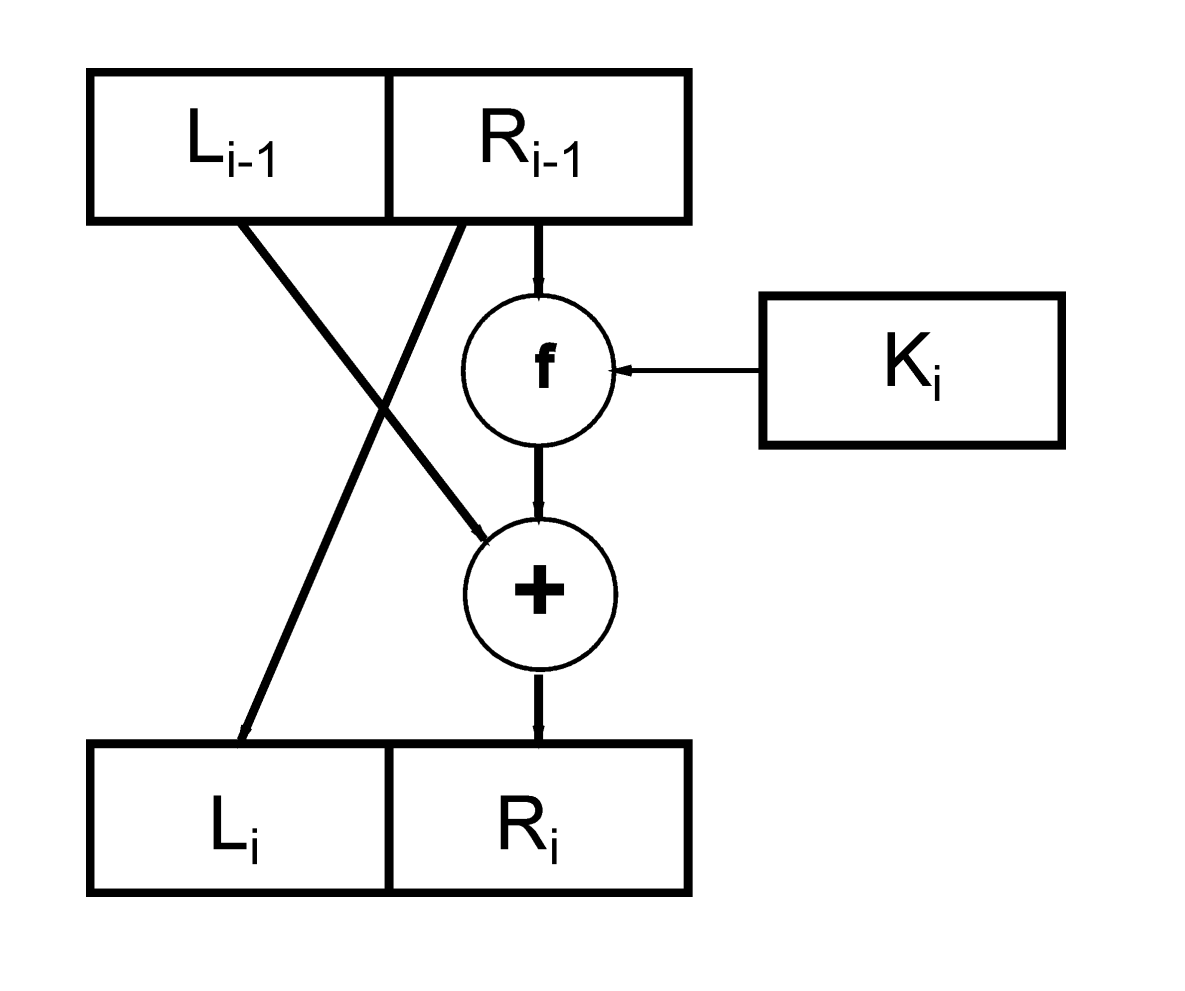
\includegraphics{img/feistel.png}}
\end{center}

\textit{Kodiranje}
\begin{koda}
$L_0 = $ leva polovica $b$
$R_0 = $ desna polovica $b$
za $i = 1, \dots, N_r$:
	$L_i = R_{i-1}$
	$R_i = L_{i-1} \oplus f_{K_i}(R_{i-1})$
$c = R_{N_r} \| L_{N_r}$
\end{koda}

\subsection*{DES in AES}
TO-DO!

\section*{Tokovne šifre}
Besedilo $b$ razdelimo na bloke $b = b_1 \dots b_t \in \mathcal{B}^t$.

Imamo zaporedje (tok) ključev: $z_1, z_2, \dots \in \mathcal{K}$.

\textit{Kodiranje}
\begin{koda}
za $j = 1, \dots, t$:
	$c_j = E_{z_j}(b_j)$
$c = c_1 c_2 \dots c_t \in \mathcal{C}^t$
\end{koda}

\textit{Dekodiranje}
\begin{koda}
za $j = 1, \dots, t$:
	$b_j = D_{z_j}(c_j)$
$b = b_1 b_2 \dots c_t \in \mathcal{B}^t$
\end{koda}

\subsection*{Aditivne tokovne šifre}
Naj bo $(G, +)$ grupa, $\mathcal{B} = \mathcal{C} = \mathcal{K}$ in $z_1, z_2, \dots$ tok ključev.

\textit{Kodiranje}
\begin{align*}
E_{z_i} (b_i) &= b_i + z_i \\	
D_{z_i} (c_i) &= c_i - z_i
\end{align*}

\subsection*{Samokodirna šifra}
$\mathcal{B} = \mathcal{C} = \mathcal{K} = \mathbb{Z}_{26}$

Začetni ključ izberemo $z_1 \in \mathbb{Z}_{26}$
\[ z_i = b_{i-1} \quad \text{za }\ i > 1 \]

\textit{Kodiranje}
\[ E_{Z_i}(b_i) = b_i + z_i \]

\textit{Dekodiranje}
\[ D_{Z_i}(c_i) = c_i - z_i \]

\subsection*{Vermanova šifra}
$\mathcal{B} = \mathcal{C} = \mathcal{K} = \{0, 1\}^n$, ključ izberemo naključno.

\textit{Kodiranje}
\[ E_k(b) = b \oplus k \]
\textit{Dekodiranje}
\[ D_k(c) = c \oplus k \]

\textit{To je pravzaprav Vigenerjeva šifra, le da ima ključ enako dolžino kot besedilo}

\textit{Uporabimo kratko seme za generiranje dolgega toka psevdonaključnih bitov, ki jih uporabimo za ključ.}

\subsection*{Linearna rekurzivna šifra}
je sinhrona tokovna šifra, pri kateri je
\[ \mathcal{B} = \mathcal{C} = \mathcal{K} = \mathbb{Z}_s\]
zaporedje ključev z linearno rekurzinvo enačbo reda $m$ s konstantnimi koeficienti nad $\mathbb{Z}_s$:
\[ z_i = c_1 z_{i-1} + c_2 z_{i-2} + \dots + c_m z_{i_m} \mod s \]
Zaporedju lahko priredimo polinom:
\[ C(x) = 1 + \sum_{i=1}^m c_i x^i \mod s\]

\textit{Kodiranje/Dekodiranje:}
\begin{align*}
	E_{z_i}(x_i) &= x_i + z_i \mod s \\
	D_{z_i}(y_i) &= y_i - z_i \mod s
\end{align*}

Perioda LFSR reda $m$ je največ $2^m - 1$

Red nerazcepnega polinoma $f(x)$ je najmanjši $t$, da $f(x) | x^t - 1$.

Če ima LFSR nerazcepen karakteristični polinom reda $t$, potem ima LFSR periodo $t$.

\subsection*{Pomični register z linearno povratno zanko}
V pomičnem registru je na začetku inicializacijski vektor $(z_1 z_2 \dots z_m)$ (ključ).

\begin{center}
	\resizebox*{0.9\columnwidth}{!}{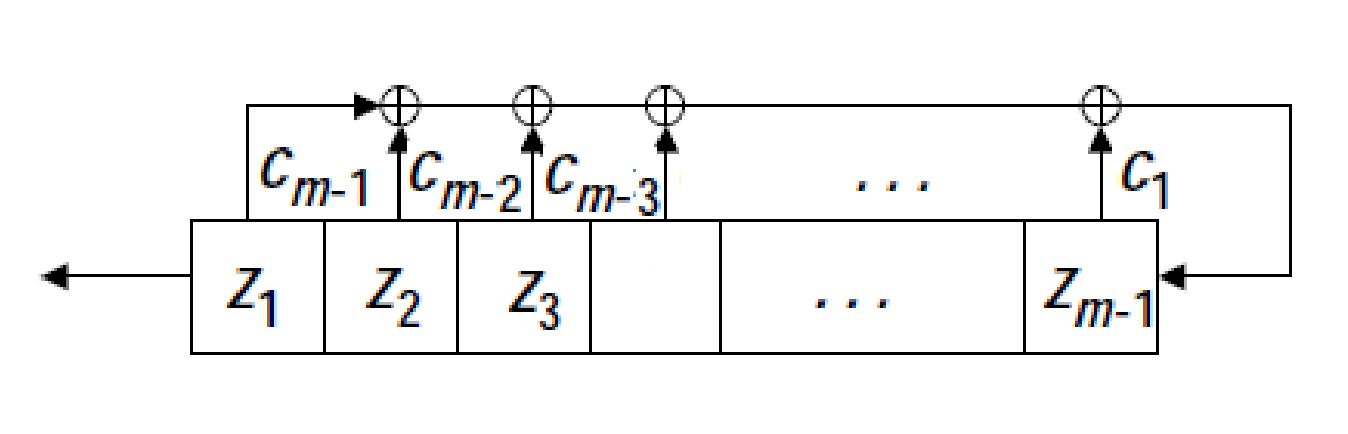
\includegraphics{img/lfsr.png}}
\end{center}

Na vsakem koraku izpišemo $z_1$ register pomaknemo v levo zadnji bit $z_m$ pa 
izračunamo kot z $c_1, \dots, c_m$ uteženo vsoto.

Če poznamo $z_0, \dots, z_{2m-1}$, lahko rešimo sistem:
\[
\begin{bmatrix}
	z_0 & z_1 & \dots & z_{m-1} \\
	z_1 & z_2 & \dots & z_{m-2} \\
	\vdots & \vdots & & \vdots \\
	z_{m-1} & z_{m} & \dots & z_{2m_2} 
\end{bmatrix}
\begin{bmatrix}
	c_m \\
	c_{m-1} \\
	\vdots \\
	c_1
\end{bmatrix}
=
\begin{bmatrix}
	z_m \\
	z_{m+1} \\
	\vdots \\
	z_{2m-1}
\end{bmatrix}
\]
Če smo pravilno uganili red $m$ ima sistem enolično rešitev.

\section*{Asimetrična kriptografija}
\subsection*{RSA}
$n = pq$ kjer sta $p$ in $q$ različni veliki praštevili.

$m = \varphi(n) = (p-1)(q-1)$

Potem je kriptosistem podan z:
\begin{align*}
	\mathcal{B} &= \mathcal{C} = \mathbb{Z}_n \\
	\mathcal{K} &= \{n\} \times \mathbb{Z}_m^* \\
	E_{(n,e)}(x) &\equiv x^e \mod n \\
	E_{(n,d)}(y) &\equiv y^d \mod n
\end{align*}

\textit{$e$ mora biti tuj $m$}

Kodirnemu ključu $(n, e)$ pripada dekodirni ključ $(n, d)$, kjer je $d = e^{-1} \in \mathbb{Z}_m^*$

\subsection*{Problem diskretnega logaritma}
Naj bo $G$ multiplikativna grupa. Za dana $\alpha, \beta \in G$, kjer je red elementa $\alpha$ enak $n$, 
je treba poiskati takšen $x \in \{0, \dots, n-1\}$, da je
\[ \alpha^x = \beta\]
Številu $x$ rečemo diskretni logaritem elementa $\beta$ z osnovo $\alpha$.

\subsubsection*{Shanksov algoritem (veliki korak - mali korak) }
\begin{koda}
vhod: $G$ grupa, $\alpha, \beta \in G$, $n = \text{red}(\alpha)$
izhod: $x = \log_\alpha \beta$
$m = \lceil \sqrt{n} \rceil$
za $j = 0, \dots, m-1$:
	$(j, \alpha^{m-j}) \to L_1$
uredi $L_1$ po drugi komponenti
za $i = 0, \dots, m-1$:
	$(i, \beta \alpha^{-i}) \to L_2$
uredi $L_2$ po drugi komponenti
poisci $(j, y) \in L_1$ in $(i, y) \in L_2$
$x = (mj + i)$
vrni $x$
\end{koda}

\subsection*{Diffie-Hellmanova izmenjava ključev}
\begin{itemize}
	\item Alenka in Bojan se dogovorita za veliko praštevilo $p$ in $\alpha \in \mathbb{Z}_p^*$, ki ima velik red $n$.
	\item Alenka si izbere naključno število $a \in \{1, \dots, n-1\}$,
	izračuna $A = \alpha^a \mod p$ in pošlje $A$ Bojanu.
	\item Bojan si izbere naključno število $b \in \{1, \dots, n-1\}$, 
	izračuna $B = \alpha^b \mod p$ in pošlje $B$ Alenki.
	\item Alenka in bojan vsak zase izračunata skupni tajni ključ $K = \alpha^{ab} = A^b = B^a$
\end{itemize}
\textit{Varnost temelji na težavnosti diskretnega logaritma.}

\textit{Zaradi možnosti napada srednjega moža je pri izmenjavi ključev nujna avtentikacija!}

\subsection*{ElGamalov kriptosistem}
\begin{itemize}
	\item Alenka in Bojan izmenjata tajni ključ k z Diffie-Hellmanovo shemo
	\item Alenka želi poslati sporočilo $x$. Izračuna kriptogram $y = k\cdot x \mod p$ in ga pošlje Bojanu.
	\item Bojan izračuna $x = k^{-1} \cdot y \mod p$
\end{itemize}
Formalna definicija:
\begin{align*}
	\mathcal{B} &= \mathcal{C} = \mathbb{Z}_p^* \\
	\mathcal{K} &= \mathbb{Z}_p^* \times \mathbb{Z}_p^* \\
	E_{(a,B)}(x) &\equiv B^a \cdot x \mod p \\
	D_{(b,A)}(y) &\equiv A^{p-b-1} \cdot y \mod p \\
\end{align*}

Naj bo $B = \alpha^b \mod p$ in $A = \alpha^a \mod p$. Potem kodirnemu kjluču $(a, B)$ ustreza dekodirni ključ $(b, A)$.

\section*{Zgoščevalne funkcije}
Zgoščevalna funkcija besedilu poljubne dolžine kratek izvleček.

Želene lastnosti:
\begin{itemize}
	\item \textbf{Naključnost}: Če se dve sporočili razlikujeta na enem samem mestu morata povzetka izgledati kot neodvisno izbrani naključni števili.
	\item \textbf{Odpornost praslik}: za poljuben izvleček $z$ je računsko nemogoče poiskati sporočilo $x$, ja je $h(x) = z$. Oz. zgoščevalna funkcija je \textbf{enosmerna}.
	\item \textbf{Odpornost drugih praslik}: za dano sporočilo $x$ je nemogoče najti drugo sporočilo $x'$, ki ima enak izvleček.
	\item \textbf{Odpornost na trke}: računsko je nemogoče poiskati dve različni sporočili $x$ in $x'$ z enakim povzetkom.
\end{itemize}
\textbf{Trk} je par različnih sporočil z enakim povzetkom.

\subsection*{Tipična zgoščevalna funkcija}
\begin{itemize}
	\item \textbf{Komprsijska funkcija}: $f: \{0,1\}^{r+n} \to \{0,1\}^n$
	\item \textbf{Zgoščevalna funkcija}: $h: \{0,1\}^* \to \{0,1\}^n$
\end{itemize}

Zgoščevalna funkcija iterativno kliče kompresijsko funkcijo.

\begin{koda}
$H_0 = IV$
za $i = 1, \dots, t$:
	$H_i = f(H_{i-1} \| x_i)$
$h(x) = H_t$
\end{koda}

Tukaj je $IV$ začetno stanje, $x_i$ pa so bloki besedila.

Na konec besedila dodano nekaj bitov, ki popisujejo dolžino besedila in toliko ničel, da se besedilo lahko razdeli na enako velike bloke.

\textit{Če je kompresijska funkcija odporna na trke, je tudi zgoščevalna funkcija odporna na trke.}


\section*{Digitalni podpisi}
Formalno je \textbf{sistem na digitalno podpisovanje} peterka $(\mathcal{B}, \mathcal{A}, \mathcal{K}, \mathcal{S}, \mathcal{V})$, kjer je
\begin{itemize}
	\item $\mathcal{B}$ končna množica sporočil
	\item $\mathcal{A}$ končna množica podpisov
	\item $\mathcal{K}$ končna množica ključev
	\item za vsak ključ $K \in \mathcal{K}$ obstaja algoritem za podpisovanje in preverjanje podpisa
	\[ \text{sig}_K \in S, \qquad \text{sig}_K : \mathcal{B} \to \mathcal{A} \]
	\[ \text{ver}_K \in S, \qquad \text{ver}_K : \mathcal{B} \times \mathcal{A} \to \{\text{true}, \text{false}\} \]
\end{itemize}
Algoritem za podpisovanje je znan le podpisniku.

\subsection*{Podpisovanje z algoritmom RSA}
Naj bosta $p, q$ praštevili in $n = pq$. Naj bo $(n, d)$ zasebni in $(n, e)$ javni ključ.
Potem za $K = (n, e, d)$ definiramo:
\begin{align*}
\text{sig}_K(x) &= x^d \mod n \\
\text{ver}_K(x,y) &= \left( \text{true} \iff x = y^e \mod n \right)
\end{align*}

\subsection*{ElGamalov sistem za digitalno podpisovanje}
\subsubsection*{Generiranje ključa}
Naj bo $p$ takšno praštevilo, ja je v $\mathbb{Z}$ težko izračunati diskretni logaritem in $\alpha \in \mathbb{Z}_p^*$ primitivni element.

Potem je $\mathcal{B} = \mathbb{Z}_p^*$, $\mathcal{A} = \mathbb{Z}_p^* \times \mathbb{Z}_{p-1}$ in 
$\mathcal{K} = \{(p, \alpha, a, \beta) : \beta \equiv \alpha^a \mod p \}$.

Število $a$ je zasebno. Števila $p$, $\alpha$ in $\beta$ pa so javna.

\subsubsection*{Podpisovanje}
Podpisnik s ključem $K = (p, \alpha, a, \beta)$ izbere naključno skriteo število $k \in \mathbb{Z}_{p-1}^*$ in določi
\[ \text{sig}_K(x, k) = (\gamma, \delta)\]
kjer je
\begin{align*}
	\gamma &\equiv \alpha^k \mod p \\
	\delta &\equiv (x - a\gamma) k^{-1} \mod p
\end{align*}

\subsubsection*{Preverjanje podpisa}
Za to potrebujemo $p$, $\alpha$ in $\beta$, ki so javni:
\[ \text{ver}_K(x, \gamma, \delta) = \left( \text{true} \iff \beta^\gamma \gamma^\delta \equiv_p \alpha^x \right)\]

\subsection*{Digital Signature Standard (DSA)}
\subsubsection*{Generiranje ključa}
\begin{itemize}
	\item Izberi 160-bitno praštevilo $q$
	\item Izberi 1024-bitno praštevilo $p$, da $q|(p-1)$
	\item Izberi element $h \in \mathbb{Z}_p^*$ in izračunaj $\alpha = h^{(p-1)/q} \mod p$; ponavljaj dokler $\alpha \neq 1$. ($\alpha$ je generator natanko določen ciklične grupe red $q$ v $\mathbb{Z}_p^*$)
	\item Izberi naključno naravno število $a < q$
	\item Izračunaj $\beta = \alpha^a \mod p$
	\item Janvi ključ osebe $A$ je $(p, q, \alpha, \beta)$, zasebni pa $a$.
\end{itemize}
\textit{Opomba:} red $\alpha, \beta, \gamma$ je enak $q$.

\subsubsection*{Podpisovanje}
\begin{itemize}
	\item Izberi naključno naravno število $k$, ki je manjše od $q$.
	\item Izračunaj $\gamma = \left( \alpha^k \mod p\right) \mod q$
	\item Izračunaj $k^{-1} \mod q$.
	\item Izračunaj $\delta = k^{-1}(h(x) + a\gamma) \mod q$, kjer je $h(x)$ povzetek sporočila $x$, dobljen z zgoščevalno funkcijo SHA-1.
	\item Če je $\gamma = 0$ ali $\delta = 0$, začni ponovno.
	\item Podpis sporočila je $(\gamma, \delta)$.
\end{itemize}

\subsubsection*{Preverjanje podpisa}
\begin{itemize}
	\item Priskirbi si overjeno kopijo javnega kjluča $(p,q,\alpha,\beta)$ podpisnika
	\item Izračunaj $w = \delta^{-1} \mod q$ in $h(x)$
	\item Izračunaj $e_1 = h(x)w \mod q$ in $e_2 = \gamma w \mod q$
	\item Izračunaj $v = (\alpha^{e_1} \beta^{e_2} \mod p ) \mod q $
	\item Sprejmi podpis, če je $v = \gamma$
\end{itemize}


\section*{Uporaba bločnih šifer}
\subsection*{Elektronska kodna knjiga (ECB)}
Naivni način uporabe bločnih šifer. Z istim klučem kodiramo zaporedoma bolk po blok.

\begin{align*}
	c_i &= E_k(b_i) \\
	b_i &= D_k(c_i)
\end{align*}

\subsection*{Veriženje kodnih blokov (CBC)}
Izberemo inicializacijski vektor $IV$ dolžine $n$.

\textit{Kodiranje}
\begin{koda}
$c_0 = IV$
za $j = 1, \dots, m$:
	$c_j = E_e(b_j \oplus c_{j-1})$
$c = c_1  \dots c_m$
\end{koda}

\textit{Dekodiraje}
\begin{koda}
$c_0 = IV$
za $j = 1, \dots, m$:
	$b_j = D_e(c_j) \oplus c_{j-1}$
$b = b_1  \dots b_m$
\end{koda}

Napaka na bloku $c_j$ vpliva le na $b_j$ in $b_{j+1}$

\subsection*{Način s števcem (CM)}
Izberemo števec $ctr$ dolžine $n$. Besedilo razdelimo na bloke dolžine $n$: $b = b_1 \dots b_m$.

\textit{Kodiranje}
\begin{koda}
za $ j = 1, \dots, m$:
	$l_j = ctr + j - 1 \mod 2^n$
	$c_j = b_j \oplus E_e(l_j)$
$c = c_1 \dots c_m$
\end{koda}

\textit{Dekodiranje}
\begin{koda}
za $ j = 1, \dots, m$:
	$l_j = ctr + j - 1 \mod 2^n$
	$b_j = c_j \oplus E_e(l_j)$
$b = b_1 \dots b_m$
\end{koda}

\section*{Napadi na kriptosisteme}
\subsection*{Pasivni napadi}
\begin{itemize}
	\item \textbf{Napad za golim kriptogramom}: nasprotnik pozna enega ali več kriptogramov.
	\item \textbf{Napad z znanim besedilom}: nasprotnik pozna enega ali več parov (besedilo, kriptogram).
	\item \textbf{Napad z izbranim besedilom}: nasprotnik ima začasen dostop do kodirnega postopka. Generira pare $(b,c)$ za izbrana besedila $b$. \textit{V primeru kriptosistemov z javnimi ključi tak napad štejemo za paseiven.}
\end{itemize}

\subsection*{Aktivni napadi}
\begin{itemize}
	\item \textbf{Napd z izbranim kriptogramom}: nasprotnik za izbrane kriptograme lahko zahteva ustrezna besedila. Kasneje dobi kriptogram $c$, ki ga želi dekodirat.
	\item \textbf{Prilagodljivi napad z izbranim kriptogramom}: nasprotnik skuša dešifirati $c$ med tem lahko za izbrane kriptograme lahko zahteva ustrezna besedila.
\end{itemize}

\subsection*{Stopnje varnosti}
\begin{itemize}
	\item \textbf{Brezpogojna varnost}: tudi če ima napadalec neomejene računske vire, samo iz kriptograma na izve nobene informacije o besedilu (razen dolžine)
	\item \textbf{Semantična varnost}: napadalec s polinomsko omejenimi viri samo iz kriptograma z nezanemarljivo verjetnostjo ne izve nobene informacije o besedilu (razen dolžine).
	\item \textbf{Polinomska varnost}: napadalec s polinomsko omejenimi viri z nezanemarljivo verjetnostjo ne more ločiti med kriptogramoma danih besedil iste dolžine.
\end{itemize}
\textit{Za pasivnega napadalca sta semantična in polinomska varnost ekvivalentni.}

\subsection*{Sistemi s popolno tajnostjo (LPT)}
Simetrični kriptosistem $\mathcal{S} = (\mathcal{B}, \mathcal{C}, \mathcal{K}, \mathcal{E}, \mathcal{D})$ opremimo
z verjetnostno porazdelitvijo na množici $\mathcal{B} \times \mathcal{K}$

\begin{align*}
	B \quad &\dots \quad \text{slučajna sprem. z zalogo vrednosti } \mathcal{B} \\
	K \quad &\dots \quad \text{slučajna sprem. z zalogo vrednosti } \mathcal{K} \\
	C \quad &\dots \quad \text{slučajna sprem. z zalogo vrednosti } \mathcal{C} \\
\end{align*}
$C$ je določena z $B$ in $K$

Predpostavimo, da st $B$ in $K$ neodvisni:
\[ P(B = b \cap K = k) = P(B = b) P(K = k) \]
za vsak $b \in \mathbb{B}$ in vsak $c \in \mathcal{C}$ velja še:
\[ P(B = b) > 0 \quad \text{oziroma} \quad P(C = c) > 0 \]

Potem ima kriptosistem $S$ \textbf{lastnost popolne tajnosti} natanko tedaj, ko
\[ \forall b \in \mathcal{B}, c \in \mathcal{C}: \ P(B = b | C = c) = P(B = b)\]

Vrednost $C$ za dana $b \in \mathcal{B}$ in $k \in \mathcal{K}$ je:
\[ c = E_k(b) \]

Verjetnost dogodka $(C = c)$ dobimo iz formule za popolno verjetnost:
\[ P(C = c) = \sum_{b \in \mathcal{B}} P(C = c | B = v) P(B = b) \]
\[ P(C = c | B = b) = \sum_{k \in \mathcal{K}:\ E_k(b) = c} P(K = k) \]

\subsubsection*{Verjetnostne formule}
\begin{align*}
	P(A|B) &= \frac{P(A \cap B)}{P(B)} & P(A|B) &= \frac{P(B|A)P(A)}{P(B)} 
\end{align*}

\textit{Trditev:} Če ima kriptosistem lastnost popolne tajnosti, za 
vsak $b \in \mathcal{B}$ in $c \in \mathcal{C}$ obstajaj $k \in \mathcal{K}$, 
da velja $E_k(b) = c$. In $|\mathcal{B}| \leq |\mathcal{C}| \leq |\mathcal{K}|$


\textit{Izrek (Shannon):} Naj velja $|\mathcal{B}| = |\mathcal{C}| = |\mathcal{K}|$.
Potem ima kriptosistem $S$ lastnost popolne tajnosti natanko tedaj, ko
\begin{itemize}
	\item za vsak $b \in \mathcal{B}$ in vsak $c \in \mathcal{C}$ obstaja en $k \in \mathcal{K}$,
	da je $E_k(b) = c$
	\item slučajna spremnljivka $K$ je enakomerno porazdeljena.
\end{itemize}

\section*{Teorija števil}

\subsection{Eulerjeva funkcija}
Eulerjeva funkcija nam pove koliko je obrnlivih elementov v $\mathbb{Z}_m$.

\[ | \mathbb{Z}_m^* | = \varphi(m) \]

Za $n \in \mathbb{N}$ s paraštevilskim razcepom \\ $ n = p_1^{\alpha_1} \cdot ... \cdot p_m^{\alpha_m}$ velja:
\[\varphi(n) = \varphi(p_1^{\alpha_1}) \cdot ... \cdot \varphi(p_m^{\alpha_m}) = n \prod_{ p_k \in \mathbb{P}} \left(1-\frac{1}{p_k} \right) \]

\textbf{Euljerjev izrek:}

Naj bo $G$ končna grupa. Potem red elementa $a \in G$ deli red grupe $G$.

\[\textrm{gcd}(a, m) = 1 \Leftrightarrow a^{\varphi(m)} \equiv_m 1; a \in \mathbb{Z}_m^*\]
\[a,m \in \mathbb{N} \wedge \textrm{gcd}(a, m) = 1 \Rightarrow a^{\varphi(m)} \equiv_m 1\]
\[a^{\varphi(m)} = 1 \text{ v } \mathbb{Z}_m^*\]

\textbf{Mali Fermatov izrek:} če je $m \in \mathbb{P}$ ($\varphi(m) = m-1$) in $\textrm{gcd}(a,m) = 1$, potem:
\[a^{m-1} \equiv_m 1\]

\textbf{Fermantov test praštevilskosti}
$p$ praštevilo $\implies$ $a^{p-1} \equiv_p 1$

Če želimo preveriti ali je $p$ praštevilo, zgornjo trditev preizkusimo za nekaj naključnih $a$-jev.

\subsection{Linearne diofantske enačbe}
Diofantska enačba $ax + by = c$ ima rešitev $\Leftrightarrow$ $gcd(a, b) | c$. 

Če ima eno rešitev $(x_0, y_0) \in \mathbb{Z}^2$ ima neskončno množico rešitev:
\[\{(x_k, y_k) : k \in \mathbb{Z}\}\]
\[x_k = x_0 - k\frac{b}{\textrm{gcd(a, b)}}\]
\[y_k = y_0 + k\frac{a}{\textrm{gcd(a, b)}}\]

\subsubsection*{Razširjen evklidov algoritem}

\begin{koda}
vhod: $(a, b)$
($r_0$, $x_0$, $y_0$) = ($a$, 1, 0)
($r_1$, $x_1$, $y_1$) = ($b$, 0, 1)
$i$ = 1

dokler $r_i$ $\neq$ 0:
    $i$ = $i$+1
    $k_i$ = $r_{i-2} // r_{i-1}$
    $(r_i, x_i, y_i)$ = $(r_{i-2}, x_{i-2}, y_{i-2}) - k_i(r_{i-1}, x_{i-1}, y_{i-1})$
konec zanke
vrni: $(r_{i-1}, x_{i-1}, y_{i-1})$
\end{koda}

Naj bosta $a, b \in \mathbb{Z}$. Tedaj trojica $(d, x, y)$, ki jo vrne razširjen evklidov algoritem z vhodnim podatkomk $(a, b)$, zadošča:
\[ax + by = d \text{ in } d = \textrm{gcd}(a, b)\] 


\subsection*{Grupe}
\begin{itemize}
    \item \textbf{grupoid} $(M, \cdot)$ urejen par z neprazno množico $M$ in zaprto opreacijo $\cdot$.
    \item \textbf{polgrupa} grupoid z asociativno operacijo $ \forall x,y,z \in M : (x\cdot y)\cdot z = x\cdot (y\cdot z)$.
    \item \textbf{monoid} polgrupa z enoto $ \exists e \in M \ \forall x \in M : e\cdot x = x\cdot e = x$.
    \item \textbf{grupa} polgrupa v kateri ima vsak element inverz $ \forall x \in M \ \exists x^{-1} \in M : x\cdot x^{-1} = x^{-1}\cdot x = e$.
    \item \textbf{abelova grupa} grupa s komutativno operacijo $ \forall x,y \in M  : x\cdot y = y\cdot x$.
\end{itemize} 

\subsubsection{Množica $\mathbb{Z}_m$}
$\mathbb{Z}_m = \{0,1,...,m-1\}$

Vpeljemo seštevanje $+_m$ po modulu $m$ in množenje $\cdot_m$ po modulu $m$. 
Dobimo grupo $(\mathbb{Z}_m, +_m)$ in monoid $(\mathbb{Z}_m, \cdot_m)$.

Red elementa $x\in \mathbb{Z}_m$ je $\frac{m}{\gcd(m,x)}$

\subsubsection{Množica $\mathbb{Z}_m^*$}
To je množica vseh obrnljivih elementov v $\mathbb{Z}_m$ (operacija: množenje).
\[|\mathbb{Z}^*_m| = \varphi(m)\]
Element $x\in \mathbb{Z}_m$ je obrnljiv če se da rešiti \emph{diofantsko enačbo}:
\[ xy + km = 1\]
za neznanki $y$ (inverz od $x$) in $k$.

\subsubsection{Cayleyjeva tabela}
Za vsak element množice imamo en stolpec in eno vrstico. V vsakem polju je produkt elementa vrstice in elementa stolpca.
(Presek vrstice $a$ in stolpca $b$ je $ab$)

\subsubsection{Red elementa}
Naj bo $(G,\cdot)$ grupa. Red elemneta $a$ je najmanjše naravno število $n \in \mathbb{N}$, da velja
\[a^n = e\]
\textit{oznaka:} $\#a$

\subsubsection{Red grupe}
je število elementov $G$, oznaka $|G|$.

\subsubsection*{Ciklična grupa}
Grupa je ciklična, če vsebuje $a$ reda $|G|$:
\[ G = \left\{ a, a^2, a^3, \dots, a^{|G|} = e\right\}\]


\[ \text{red}_{\mathbb{Z}_p^*}(\alpha^i) = \text{red}_{\mathbb{Z}_p^*}(i) = \frac{p-1}{\gcd(i, p-1)}\]

$x$ je generator grupe $\mathbb{Z}^*_p$ $\iff$ $\# x = p - 1$

$x$ je generator grupe $\mathbb{Z}^*_p$ $\iff$ $x^{\frac{p-1}{p_i}} \neq 1 \mod p$, za vsak $i$, jer je $p-1 = p_1^{k_1} \dots p_l^{k_l}$.

\subsection*{Končni obsegi}
$(K, +,\cdot)$ je obseg, če je
\begin{itemize}
	\item $(K, +)$ abelova grupa
	\item $(K^*, \cdot)$ grupa ($K^* = K \setminus \{0\}$)
	\item velja distributivnost:
	\[ a \cdot (b+c) = (a\cdot b) + (a \cdot c)\]
	\[ (a+b) \cdot c = (a\cdot c) + (b \cdot c)\]
\end{itemize}

Obseg je \textbf{komutativen}, če je $(K^*, \cdot)$ komutativna.

\subsection*{Praštevilski obsegi}
Če je $p$ praštevilo, je $(\mathbb{Z}_p, +_p, \cdot_p)$ končen obseg.


\subsection*{Galoisovi obsegi}
\[\text{GF}(p) \cong \mathbb{Z}_p \qquad p \in \mathbb{P}\]
\[ \text{GF}(p^n) \cong \mathbb{Z}_p[x]/(u) \]
\begin{itemize}
	\item $u \in \mathbb{Z}_p[x]$ je nerazcepen polinom stopnje $n$
	\item elementi $\text{GF}(p^n)$ so ostanki polinomov iz $\mathbb{Z}_p$ pri deljenju z polinomom $u$
	\item seštevanje je enako kot seštevanje v $\mathbb{Z}_p[x]$
	\item produkt izračunamo v $\mathbb{Z}_p[x]$ nato pa vzamemo ostanek pri deljenju z $u$
\end{itemize}

Množica neničelnih/obrnljivih elementov $(GF(p^n)^*, \cdot) \cong (\mathbb{Z}_{p^n-1}, \cdot)$ je vedno izomorfna neki ciklični grupi.
Generatorjem te grupe rečemo \textbf{primitivni elementi} Galoisovega obsega.

\subsection*{Kitajski izrek o ostankih}
Naj bodo $n_1, \dots, n_k$ paroma tuja.
\begin{align*}
	x &\equiv a_1 \mod n_1 \\
	 & \vdots \\
	x &\equiv a_k \mod n_k \\
\end{align*}
\[ N = n_1 \cdot n_2 \cdot \dots \cdot n_k \]
Vse rešitve zgornjega sistema so kongurentne po modulu $N$.

\[ N_i = \frac{N}{n_i} \qquad M_i = \text{ inverz } N_i \text{ po modulu } n_i\]
\[x = \sum_{i=1}^{k} a_i M_i N_i \mod N\]

\end{multicols}
\end{document}